\documentclass[10pt]{article}
\usepackage[dvipsnames]{xcolor}
\usepackage{tikz}
\usepackage[margin=0cm]{geometry}
\pagestyle{empty}

\begin{document}

\vspace*{\fill}
\begin{center}
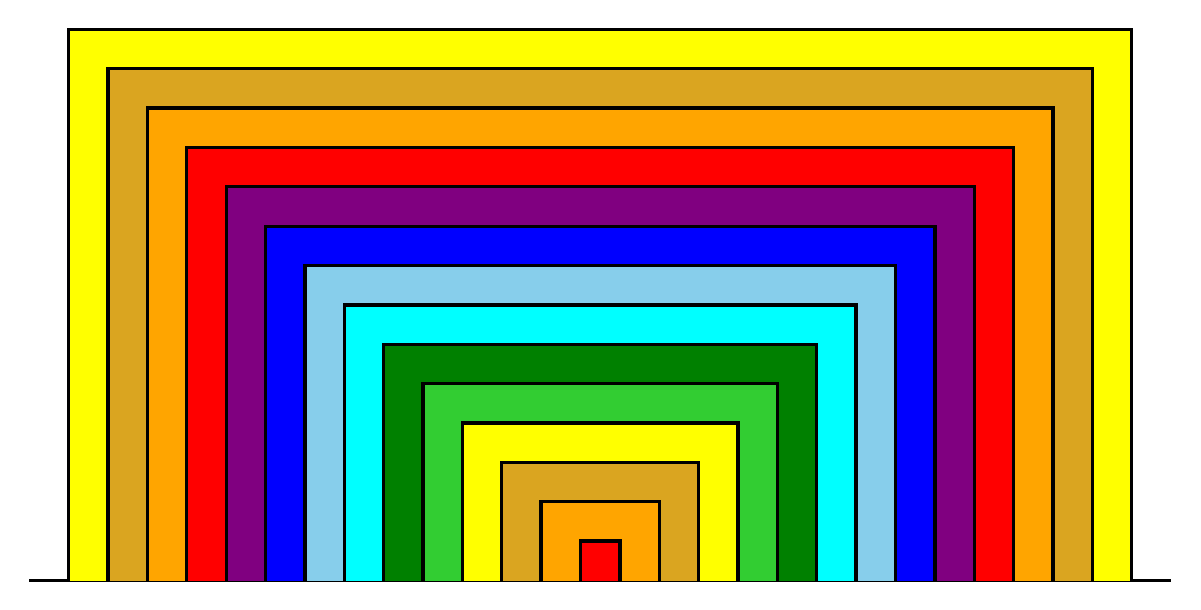
\begin{tikzpicture}[x=0.5cm, y=0.5cm, very thick]
\draw (-1,0) -- (28,0);
% Arches of depth 13
    \draw[fill=Yellow] (0,0) -- (0,14) -- (27,14) -- (27,0);
% Arches of depth 12
    \draw[fill=Goldenrod] (1,0) -- (1,13) -- (26,13) -- (26,0);
% Arches of depth 11
    \draw[fill=Orange] (2,0) -- (2,12) -- (25,12) -- (25,0);
% Arches of depth 10
    \draw[fill=Red] (3,0) -- (3,11) -- (24,11) -- (24,0);
% Arches of depth 9
    \draw[fill=Purple] (4,0) -- (4,10) -- (23,10) -- (23,0);
% Arches of depth 8
    \draw[fill=Blue] (5,0) -- (5,9) -- (22,9) -- (22,0);
% Arches of depth 7
    \draw[fill=SkyBlue] (6,0) -- (6,8) -- (21,8) -- (21,0);
% Arches of depth 6
    \draw[fill=Cyan] (7,0) -- (7,7) -- (20,7) -- (20,0);
% Arches of depth 5
    \draw[fill=Green] (8,0) -- (8,6) -- (19,6) -- (19,0);
% Arches of depth 4
    \draw[fill=LimeGreen] (9,0) -- (9,5) -- (18,5) -- (18,0);
% Arches of depth 3
    \draw[fill=Yellow] (10,0) -- (10,4) -- (17,4) -- (17,0);
% Arches of depth 2
    \draw[fill=Goldenrod] (11,0) -- (11,3) -- (16,3) -- (16,0);
% Arches of depth 1
    \draw[fill=Orange] (12,0) -- (12,2) -- (15,2) -- (15,0);
% Arches of depth 0
    \draw[fill=Red] (13,0) -- (13,1) -- (14,1) -- (14,0);
\end{tikzpicture}
\end{center}
\vspace*{\fill}

\end{document}
